\section{The Beginner's Algorithm}
\label{sec:beginner}
This section describes the easiest algorithm to remember for a human solver. The algorithm is divided into 5 different steps. Once the algorithm has been memorized, it is easy to recognize which step of the algorithm has been reached, so the correct move sequence can be applied. It is only necessary to remember a single move sequence for each step. The beginner's algorithm can however be made more efficient by remembering another somewhat similar move sequence for a few of the steps. Despite of this the beginner's algorithm is twist-wise quite inefficient, because purpose of the moves is to reach the next step instead of reaching the solved state and thereby taking a solving detour. 

\subsection{Step 1 - getting the cross}
The first step of the beginner's algorithm is to get a cross on any face. Getting a cross on a face means to align the \facelet{}s next to the center \facelet{}, so that all of the aligned \facelet{}s are of the same color, while at the same time the used edge pieces have the same color of the center \facelet{}s on each of the two faces on which they are.

\begin{wrapfigure}{R}{0.4\textwidth}
\begin{center}
	\includegraphics[width=0.35\textwidth]{input/pics/1FLCross.jpg}	
\end{center}
\caption{A first layer cross on the green face}
\label{fig:1FL-cross}
\end{wrapfigure}

The face on which the cross is being assembled is set to be the top face. An edge piece that consists of the same colors as the center piece of the top face and the center piece of the front face is placed in the bottom of the front face. With two twists of the front face the edge piece is positioned correctly in the cross. If the edge piece is oriented correctly the cube is turned (noted y) and the process is repeated until the cross is assembled. However if the piece is oriented in the wrong way the following move sequence will change it's orientation without ruining any part of the cross that may already be assembled: \\

F' U L' U' or F U' R U

\subsection{Step 2 - completing the first layer}
When the cross is completed the next step is to position the corner pieces of the first layer correctly. The first layer is set as the down face (D). A corner with a \facet{} of the color of the down face is positioned directly above it's correct  position. The correct position is between the three faces that have the same colors as the three \facet{}s of the corner piece. Once the piece is above it's correct position, the cube should be viewed in such an angle that the piece is in the upper right corner of the front face, the following move sequence is repeated until the corner piece is oriented and positioned correctly: \\
%% Some thing is wrong in the part above, turn the cube around to have U facing down.

R' D' R D \\

If the piece is above the correct position the algorithm twists the corner clock-wise and positions it in the correct position. If the piece is in the correct position the algorithm positions the piece above the correct position. The maximum number of repetitions until the piece is oriented and positioned correctly is five, because the piece can be two twists away from it's correct orientation. 
The move sequence can be performed inverted which twists the corner counter clock-wise and looks as follows: \\

D' R' D R \\

If the correct move sequence is used the maximum number of repetitions is three. If number of twists and time used is not of importance it is only necessary to remember one of them.

\begin{wrapfigure}{R}{0.4\textwidth}
\begin{center}
	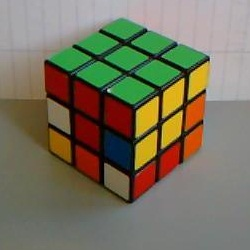
\includegraphics[width=0.35\textwidth]{input/pics/2FL.jpg}	
\end{center}
\caption{The first layer completed}
\label{fig:2FL}
\end{wrapfigure}

\subsection{Step 3 - completing the second layer}
The purpose of this step is to position the four edges belonging to the second layer correctly. The move sequence used in this step either swaps the top edge piece of the front face with the left or right edge piece. That is why the edge piece that needs to be moved down to the second layer must be positioned at the top of the face that is next to the face of one of the edges colors, where the second color is the same as the front face's color. There is however a difference in which of the two faces is used as the front face, because if the wrong face is used as front face the piece will only be positioned correctly but not oriented correctly. That \facelet{} of the edge towards the front face must be of the same color as the front face. If the edge piece is to be swapped with the right edge piece of the front face the following move sequence is used: \\

U R U' R' U' F' U F \\

If the piece is to be swapped with the left edge piece of the front face the following move sequence is used: \\

U' L' U L U F U' F' \\

If none of the edge pieces who belong to the second layer are in the third layer and the first two layers is still not completed. This occurs if the edges are all in the second layer but not positioned or oriented correctly. One of the move sequences can be used to swap an edge piece from the third layer with one of the edges in the second layer which is not positioned or oriented correctly. Now the edge piece belonging to the second layer can be moved to it's correct position.

\begin{wrapfigure}[25]{R}{0.4\textwidth}
\begin{center}
	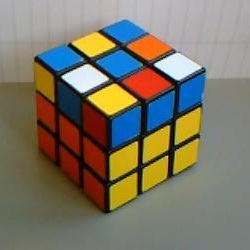
\includegraphics[width=0.35\textwidth]{input/pics/3F2L.jpg}	
\end{center}
\caption{The first two layers completed}
\label{fig:3F2L}
\end{wrapfigure}

\subsection{Step 4 - getting the last layer cross}
%%%Step 4 is divided into 4 step? Perhaps substeps instead.
Solving the last layer is divided into four steps. The order of these steps can be different and still yield the same result. We start out by getting the cross in the last layer, which is the same as the cross on the first layer. The move sequence used is however different. The only move sequence used in this step is the following: \\

F R U R' U' F' \\

Besides remembering the move sequence it is also important to know how the cube should be oriented.

If the up face colors form a line. The cube can be turned until the line forms a horizontal line. If the move sequence then is performed, the cross will be formed.

\begin{figure}[htb]
	\centering
		\subfloat[\myCaption{The up face colors form the opposite L}]{\label{fig:cross:4LLcross1}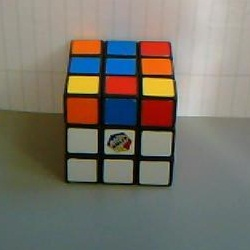
\includegraphics[width=0.28\textwidth]{input/pics/4LLcross1.jpg}}
		\hspace{0.02\textwidth}
		\subfloat[\myCaption{The up face colors form the horizontal line}]{\label{fig:cross:5LLcross2}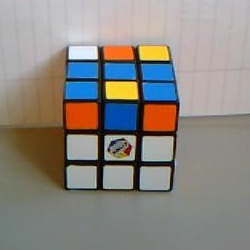
\includegraphics[width=0.28\textwidth]{input/pics/5LLcross2.jpg}}
		\hspace{0.02\textwidth}
		\subfloat[\myCaption{The up face colors form the cross}]{\label{fig:cross:6LLcross3}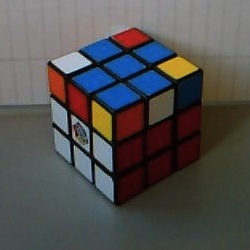
\includegraphics[width=0.28\textwidth]{input/pics/6LLcross3.jpg}}
		\caption{\myCaption{The steps in the completion of the last layer cross}}
		\label{fig:cross}
\end{figure}

If the up face colors form an opposite L character with the up face colors the move sequence will form the line. The cube must be oriented with the opposite L in the back left corner of the cube. 

If the up face colors do not form the opposite L the line or the cross, the move sequence will form the opposite L.

%Tjek om billederne st�r rigtigt
To orient the cross correctly there is one move sequence to remember: \\

R U R' U R 2U R' \\

Again it is important to know how to orient the cube. By twisting the upper layer it is possible to position the upper layer so it either has two edge pieces next to each other or directly across from each other.

\begin{wrapfigure}{R}{0.4\textwidth}
\begin{center}
	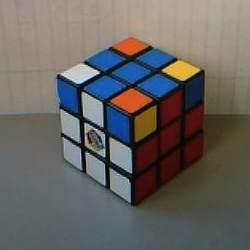
\includegraphics[width=0.35\textwidth]{input/pics/7LLedges.jpg}	
\end{center}
\caption{123}
\label{fig:7LLedges}
\end{wrapfigure}

If the correct edges piece are next to each other. The cube must be oriented with a correct edge piece on the back face and a complete face on the right face. The move sequence will then make it possible to twist the up layer so that all the edge pieces are correctly positioned and oriented.

If the correct edge pieces are across each other the move sequence can be performed a single time to get two edge pieces next to each other.


\subsection{Step 5 - completing the last layer}
The purpose of this step is to position and orient the corners correctly. Firstly the corners must be positioned correctly. To do so there are two move sequences to remember -- one for rotating three corners clockwise and one for rotating them counter-clockwise. It is however only necessary to remember one of them and repeat that one until the corners are positioned correctly, if the number of twists is unimportant to the solver. \\
\\
U R U' L' U R' U' L
\\
This move sequence will rotate the corners counter-clockwise.
\\
\\
U' L' U R U' L U R'
\\
This move sequence will rotate the corners clockwise.
\\
\\
The orientation is again important to position the corners. If one of the corners already is positioned correctly. That corner is chosen not to be moved. 

If the three other corners need to be moved counter-clockwise. The correct corner is positioned as the front right corner. The move sequence will then position the corners correctly.

If the three other corners need to be moved clockwise. The correct corner is positioned as the front left corner. The move sequence will then position the corners correctly.

If there are no correct corners. One of the two move sequences above performed once will make yield a correcly positioned corner.

\begin{wrapfigure}{R}{0.4\textwidth}
\begin{center}
	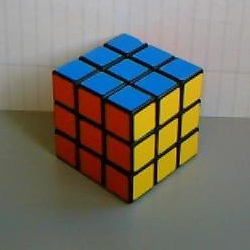
\includegraphics[width=0.35\textwidth]{input/pics/8done.jpg}	
\end{center}
\caption{123}
\label{fig:8done}
\end{wrapfigure}

To orient the corners correctly the move sequence from orienting the corners in the first layer is used: \\

R' D' R D \\

But in this step when one corner is completed. Instead of turning the whole cube to the next corner, the cube is locked on one face. Then when going to solve the next corner the upper layer is twisted until the incorrect corner is positioned at the front right corner of the cube and the move sequence is repeated.